
\documentclass[listof=totocnumbered,bibliography=totocnumbered]{scrreprt}

% imports
\usepackage[utf8]{inputenc}
\usepackage{listings}
\usepackage{cite}
\usepackage{graphicx}
\usepackage[ngerman]{babel}
\usepackage{float}
\usepackage{amsmath}
\usepackage{enumerate}
\usepackage{url}
\usepackage[font=small,format=plain,labelfont=bf,up,textfont=normal,up, justification=centering,singlelinecheck=false]{caption}
\usepackage{multirow}
\usepackage{bm} % bold in mathmode
\usepackage[binary-units=true]{siunitx} % units
\usepackage{eurosym}


% options
\setcounter{tocdepth}{2}
\numberwithin{equation}{subsection}
\renewcommand\theequation{\arabic{equation}}

% trennhilfen
\hyphenation{
er-rei-chen
}

\begin{document}
%\titlehead{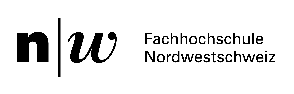
\includegraphics[scale=1]{logo.eps}}
\subject{Bachelor-Thesis}
\title{Eclipse Entwicklungsumgebung für MicroCore}
\author{Benjamin Neukom}
\date{August 2015\\\center{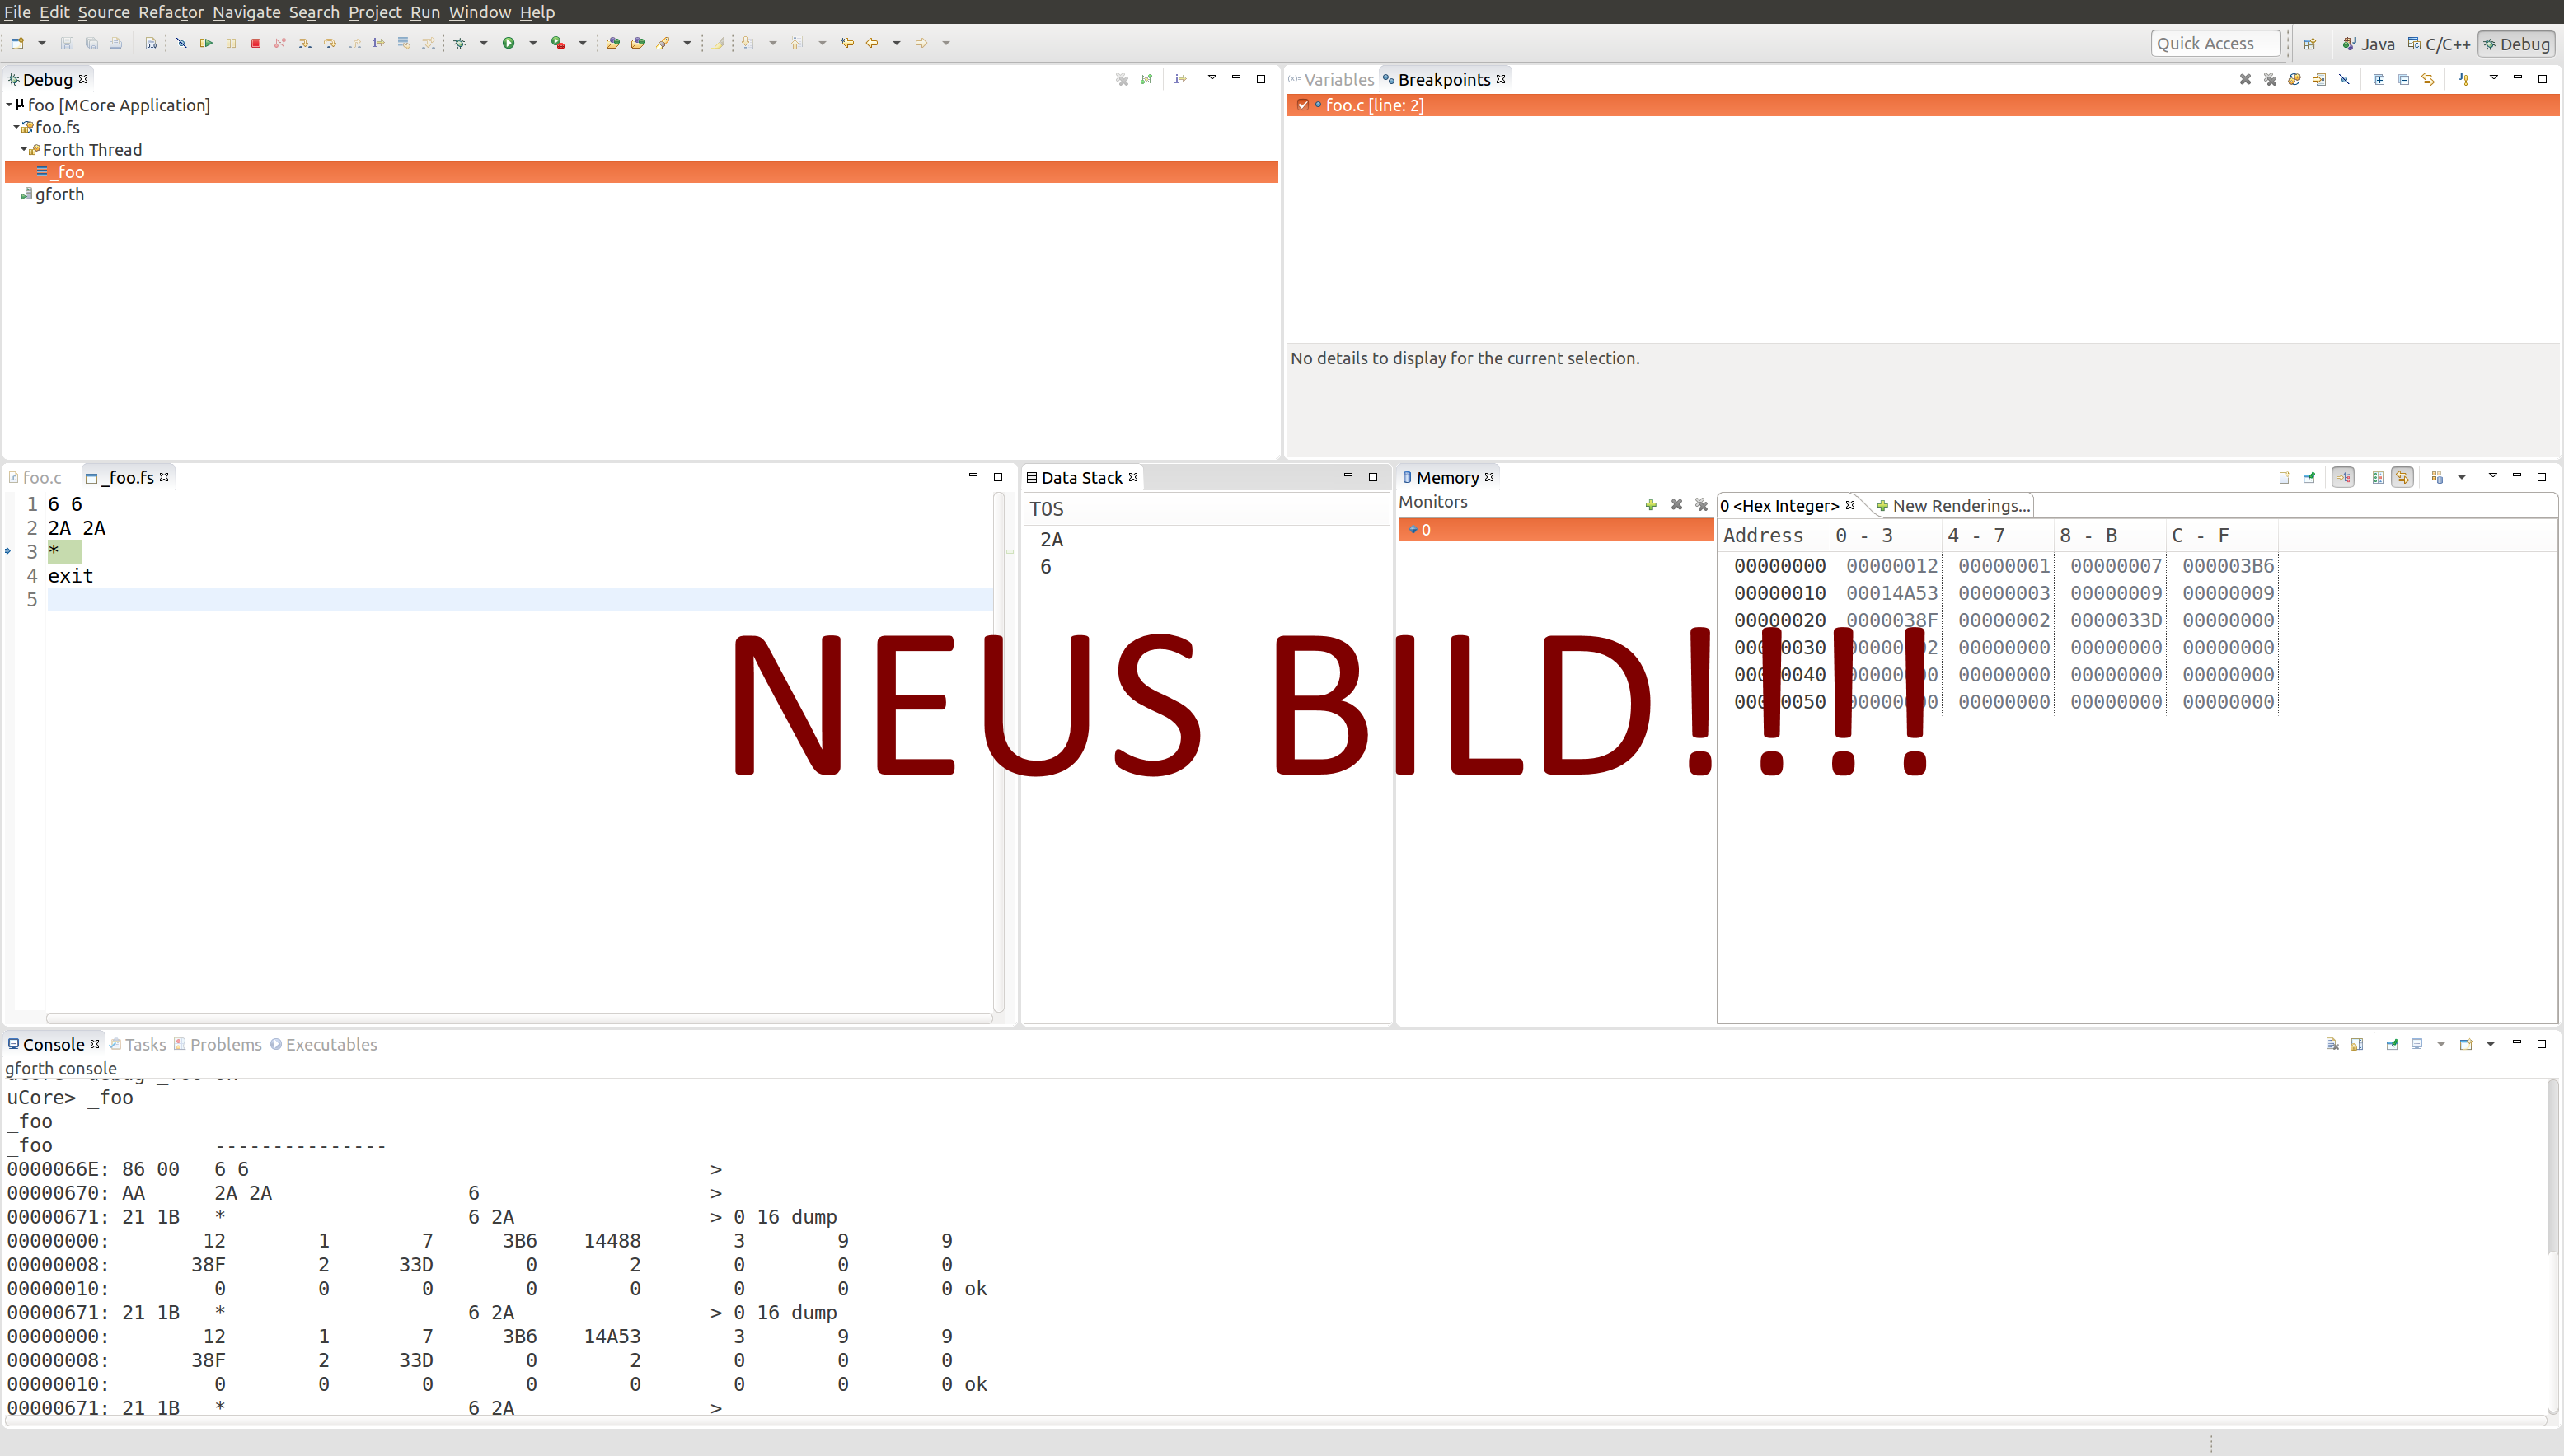
\includegraphics[scale=0.125]{title.png}}}
\publishers{Betreuer: Carlo Nicola}

\maketitle

\tableofcontents

% hauptteil
\begin{abstract}
Im ersten Teil dieser Arbeit wird beschrieben, wie eine auf Eclipse basierende Entwicklungsumgebung implementiert werden kann. Es wird gezeigt, was Eclipse für Features für Entwicklungsumgebungen bereitstellt und wie diese genutzt werden können um eine Entwicklungsumgebung darauf aufzubauen. Im zweiten Teil werden verschiedene Peephole Optimierungen für den Compiler untersucht und mit der aktuellen Peephole Implementation des Forth-Cross Compilers verglichen.
\end{abstract}

\chapter{Einleitung}

MicroCore ist eine CPU mit Harvard-Architektur, die eine Teilmenge der Forth-Sprache als Maschinensprache benutzt. MicroCore wurde in Zusammenarbeit mit der Firma Send GmbH in Hamburg entwickelt. Für die Version 1.71 wurde ein C-Compiler mit SCC (Stack-C-Compiler) implementiert. Ziel dieser Arbeit ist das Entwickeln einer auf Eclipse basierten Entwicklungsumgebung, die den SCC als Compiler verwendet. Es sollte möglich sein, den ganzen Prozess, vom Quellcode bis zur Kompilierung und dem Herunterladen auf das HW-Target in der Entwicklungsumgebung durchführen zu können. Im ersten Kapitel "`\nameref{chap:platform}"' wird beschrieben, welche Möglichkeiten Eclipse als Plattform bietet, um eine Entwicklungsumgebung zu entwickeln. Im Kapitel "`\nameref{chap:compilerintegration}"' wird erklärt, wie der Compiler integriert wurde. Im dritten Kapitel "`\nameref{chap:programlaunch}"' wird beschrieben, wie das kompilierte uForth Programm aus der Entwicklungsumgebung gestartet werden kann und was dafür implementiert wurde. Im Kapitel "`\nameref{chap:forthcommunication}"' wird beschrieben, wie die Kommunikation mit dem Forth-Prozess, entworfen, implementiert und getestet wurde. Im nächsten Kapitel "`\nameref{chap:fortheditor}"' wird beschrieben, wie Xtext dazu verwendet wurde, um einen uForth Editor in der Entwicklungsumgebung zu integrieren. Im Kapitel "`\nameref{chap:debugger}"' wird gezeigt, auf welche Arten der Debugger in die Entwicklungsumgebung eingebunden wurde und wie diese noch erweitert werden könnten. Im nächsten Kapitel "`\nameref{chap:settings}"' werden die Einstellungen, die in der Entwicklungsumgebung vorgenommen werden können, beschrieben. Im Kapitel "`\nameref{chap:optimizer}"' werden einige Peephole Optimierungen für den Compiler vorgestellt und mit der aktuellen Peephole-Optimierung des Forth-Cross-Compilers verglichen.

\chapter{Eclipse Platform}
\label{sec:EclipsePlatform}

In diesem Kapitel wird gezeigt, was Eclipse für Möglichkeiten anbietet, um eine moderne Entwicklungsumgebung zu implementieren. Diese verschiedenen Möglichkeiten werden Verglichen und die Vor- und Nachteile aufgezeigt. Es werden auch die wichtigsten Eclipse Features, welche für das Entwickeln von Eclipse Rich Client Platform (RCP) Applikationen benötigt werden, beschrieben.

\section{Eclipse als Platform}

Eclipse RCP bietet eine Basis um beliebige, (nicht zwingendermassen Entwicklungsumgebungen) Betriebssystem unabhängige Applikationen zu entwickeln. Es bietet Mechanismen, wie Plugins und Extension Points, um modulares programmieren zu unterstützen und vereinfachen. Auch bietet das Framework Features, wie das Konzept von Views und Editoren und vielem mehr, welche häufig in Applikationen gebraucht werden.

\section{Plugins}

Eclipse Applikationen nützen eine auf der OSGi Speizifikation basierten Runtime, eine Komponente in dieser Runtime ist ein Plugin. Eine Eclipse RCP Applikation besteht also aus einer Ansammlung von Plugins. Ein Eclipse Plugin ist ein Modul, welches gegen aussen ein API und Extension Points anbieten kann. 

\section{Extension Points}

Um Plugins erweitern zu können, bietet Eclipse das Konzept von Extension Points an. Über Extension Points können Plugins ein bestimmte Funktionalität anbieten, welches von anderen Plugins aufgerufen werden kann. 
\newline
So existiert zum Beispiel ein Plugin, welches einen Extension Point für Views definiert. Ein anderes Plugin kann über diesen Extension Point, deklarativ in einem XML File eine neue View erstellen. \cite{extensionpoints}

\begin{figure}[H]
	\centering
		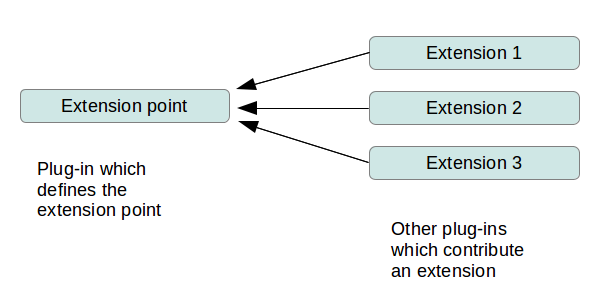
\includegraphics[scale=0.5]{platform/extensionpoint.png}
		\caption{Ein Plugin, welches einen Extension Point anbietet. Andere Plugins können}
		\captionsetup{margin=0cm,font={footnotesize}}
		\label{fig:extensionpoint}
\end{figure}

Es ist auch möglich eigene Extension Points zu definieren, falls ein eigens Plugin für andere Entwickler offen stehen soll für Erweiterungen.

\section{Eclipse basierte MCore Entwicklungsumgebung}

Eclipse als Grundlage für eine Entwicklungsumgebung zu verwenden eignet sich besonders gut, da Eclipse schon einiges an Funktionalität für eine IDE zur Verfügung stellt und schon einige Entwicklungsumgebungen mit Eclipse RCP entwickelt wurden. Auch existieren einige Tools, auf welche ich noch genauer eingehen werde, wie Xtext und DLTK, welche das entwickeln einer Entwicklungsumgebung weiter vereinfachen.

\subsection{JDT}
Eine Möglichkeit die MCore Entwicklungsumgebung zu implementieren wäre die standard Features von dem Eclipse Java Development Tools (JDT) zu verwenden. Dies wäre eine sehr Aufwändige 

\subsection{Xtext}
XText ist ein Framework, welches es erleichtert eine auf Eclipse basierte Entwicklungsumgebungen zu programmieren. Es ermöglicht auf schnelle Weise ein Grundgerüst einer IDE mit Features wie:

\begin{itemize} 
	\item Ein Editor mit Syntax Coloring
	\item Code Completion
	\item Compiler Integration
	\item Ein Java-basierter Debugger
	\item Outline
	\item Indexing
\end{itemize}

zu generieren. \cite{xtext} Es muss lediglich eine ANTLR\cite{antlr} Grammatik für die Sprache definiert werden. Der grosse Nachteil ist, dass C, inklusive Preprozessor, zu parsen sehr schwierig ist und eine Entwicklungsumgebung somit auch mit Xtext nicht einfach zu implementieren ist.

\subsection{DLTK}
Das Dynamic Language Toolkit (DLTK) ist ein weiteres Framework, welches ein Grundgerüst für eine Entwicklungsumgebungen generieren kann. Ursprünglicherweise war das Framework nur für dynamische Sprachen geignet, es kann aber auch für statische Sprachen verwendet werden. Die D Entwicklungsumgebung wurde mittels DLTK realisiert\cite{ddt}. Es bestehen aber wieder dieselben Nachteile wie bei Xtext. Da C schwierig zu parsen ist, müsste trotz dem Framework noch viel selbst implementiert werden. Da D keinen Preprozessor besitzt, konnte für diese Entwicklungsumgebung das DLTK Framework verwendet werden.

\subsection{Eclipse CDT}
Das Eclipse C-Development Tools (CDT) ist eine Eclipse Distribution mit Sprach Unterstützung für C und C++. Das CDT bietet alle Features welche man von einer Entwicklungsumgebung erwartet und stellt Extension Points zur Verfügung um diese für eine eigene Entwicklungsumgebung zu gebrauchen. So kann man mit relativ wenig Aufwand einen neues Compiler Backend in die Entwicklungsumgebung einbinden, welche den C Code kompiliert.

\subsection{Verwendung für MCore Eclipse}
Ich habe mich dazu entschieden, das Eclipse CDT als Target Platform zu wählen. Somit können alle Features, welche das Eclipse CDT zur Verfügung stellt, gebraucht werden. Frameworks, welche ein Grundgerüst einer Entwicklungsumgebung generieren, funktionieren für C nicht vollständig und sind somit keine guten Alternativen.

\chapter{Compiler Integration}
\label{compilerintegration}

In diesem Kapitel wird beschrieben, wie der Compiler in die Entwicklungsumgebung eingebunden wurde um ein C-File nach Forth zu übersetzten. Und welche Möglichkeiten mit dem CDT für das Editieren von C-Files zur Verfügung stehen.

\section{Integration im Eclipse CDT}

Das CDT stellt Extension Points zur Verfügung, welche gebraucht werden können um einen Compiler zu integrieren. Diese Extension Points werden in den nächsten Kapitel erläutert und es wird erklärt wie der LCC dadurch in die Entwicklungsumgebung eingebunden wird.

\subsection{Configuration}

Eine Konfiguration wird gebraucht um verschiedene Standard Tools und Optionen bereit zu stellen, um ein Projekt auf eine gewisse Weise zu kompilieren. Normalerweise existieren für ein Projekt zwei Konfigurationen. Eine Debug- und eine Releasekonfiguration.

\subsubsection{Verwendung}
Es gibt nur eine Konfiguration für den Release Build. Debug spezifische Files werden von dem Launch generiert, da der Kompiler damit nichts zu tun hat.

\subsection{Tool}
Definiert ein Tool, wie zum Beispiel ein Compiler oder Linker, welches verwendet wird im Buildprozess.

\subsubsection{Verwendung}
Es wird nur ein Tool verwendet, welches den LCC Compiler aufruft und somit das Forth File generiert. Für dieses Tool wurde noch eine Option (\verb!-S-Q!) definiert, welche den Peephole Optimizer deaktiviert.

\subsection{Toolchain}
Eine Liste von Tools welche gebraucht werden um den Output des Projekts zu generieren. 

\subsubsection{Verwendung}
Die Toolchain beinhaltet nur das vorhin beschriebene Tool um den LCC Compiler aufzurufen.

\subsection{CDT Builder}

TODO benennt die Forth Files um (WHY?)

\section{Project Nature}

TODO findet Errors im Path (falls Eclipse nicht richtig aufgesetzt wurde)

\chapter{Programm Launch}
\label{chap:programlaunch}
In diesem Kapitel wird beschrieben, wie das kompilierte uForth-Programm aus der Entwicklungsumgebung gestartet werden kann und was dafür implementiert wurde.

\section{Launch}

In Eclipse wird zwischen zwei Launch-Möglichkeiten unterschieden. In den nächsten Kapiteln werden die zwei Launch-Möglichkeiten erklärt.

\begin{figure}[H]
	\centering
		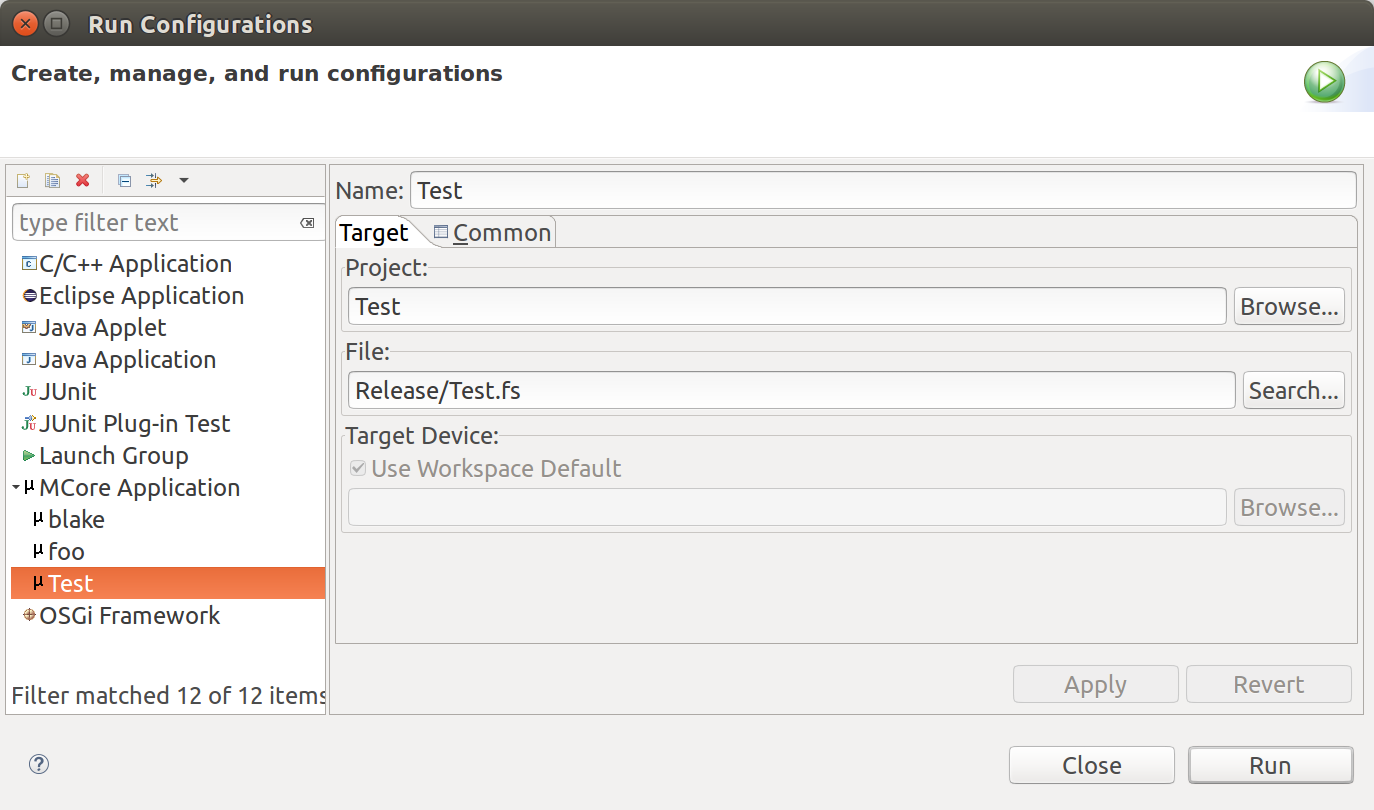
\includegraphics[scale=0.3]{launch/run.png}
		\caption{Der Launch Configuration Dialog. In diesem Dialog kann eine neue MCore Launch-Konfiguration erstellt werden. Um eine gültige Konfiguration zu erstellen, muss das Projekt und das Forth File, das gestartet werden soll, angegeben werden.}
		\captionsetup{margin=0cm,font={footnotesize}}
		\label{fig:run}
\end{figure}

\newpage
\subsection{Run}

Mit der Run-Konfiguration wird zuerst der Loader in den Forth Workspace kopiert, der in den Umgebungsvariablen definiert sein muss. Danach wird der Forth-Prozess gestartet und der Umbilical Port mittels \verb!Umbilical: /dev/ttyUSBX! gesetzt. Der Umbilical Port und der Loader müssen in der MCore Preference Page gesetzt werden (siehe Kapitel \nameref{chap:settings}). Falls der Umbilical Port ungültig ist, erscheint beim starten des Programms eine Fehlermeldung.

\begin{figure}[H]
	\centering
		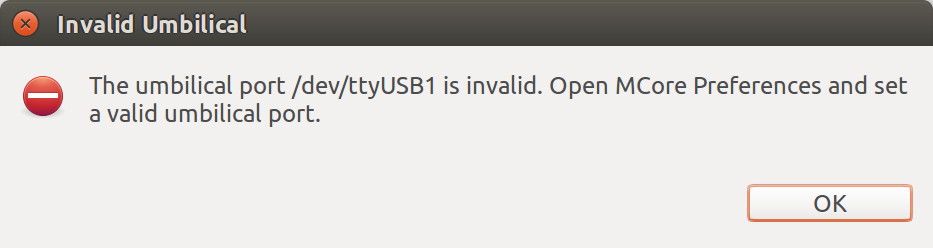
\includegraphics[scale=0.4]{launch/invalidumbilical.png}
		\caption{Dialog, der erscheint, wenn ein Programm gestartet wird und der Umbilical Port ungültig ist. Der Port kann in der MCore Preference Page geändert werden.}
		\captionsetup{margin=0cm,font={footnotesize}}
		\label{fig:invalidumbilical}
\end{figure}

\subsection{Debug}

In der Debug-Konfiguration werden zusätzlich alle Funktionen des gestarteten Forth Files disassembliert. Dies wird gemacht, damit der Debugger die Funktionen in einem File anzeigen kann. Es kann nicht der vom Compiler generierte Code genommen werden, da der Forth Cross-Compiler noch Optimierungen am Code vornimmt.


\chapter{Forth Kommunikation}
\label{forthcommunication}

In diesem Kapitel wird beschrieben wie die Entwicklungsumgebung mit dem Forth Prozess kommuniziert. Die Kommunikation mit dem Forth Prozess ist von zentraler Bedeutung, da viel der Funkionalität der Entwicklungsumgebung davon abhängt. Es wird gezeigt wie die Kommunikation designt implementiert und getestet wurde.

TODO asynchronität?


\section{Prozess Kommunikation}
Um mit dem Prozess zu kommunizieren gibt es einige Alternativen welche ich aufzeigen möchte.

\subsection{Probleme bei der Kommunikation}

TODO 

\subsection{GDB/MI-Commands}

TODO sehr komplex! (http://www.ibm.com/developerworks/library/os-eclipse-cdt-debug2/ complicated)

Eine Möglichkeit mit dem Prozess zu kommunizieren wäre ein MaschineInterface wie es der GDB macht mittels MachineInterface (MI)  Commands. GDB/MI ist ein linien basiertes Maschinen orientiertes Text Interface zu dem GDB. Es wurde dazu entwickelt um 

\subsection{Direkte Kommunikation mit dem Prozess}

\section{API Design}

In einem ersten Schritt wurde ein API designt, welches verwendet werden soll um die Kommunikation mit dem Prozess möglichst einfach zu halten.

\section{Implementierungs Details}

TODO class hi

\subsection{Kommunikation mittels Commands}

\subsection{Forth Output Parsing}

\subsection{Await auf Resultate}


\chapter{Debugger}

In diesem Kapitel wird beschrieben, wie der Debugger in Eclipse integriert wurde. Es wird aufgezeigt, was für Möglichkeiten existieren einen Debugger in Eclipse zu integrieren und welche implementiert wurden.

\section{Breakpoints}
Als erstes müssen für den Debugger Breakpoints gesetzt werden können. Dafür stehen zwei Möglichkeiten zur Verfügung, welche in den nächsten Kapiteln erläutert und verglichen werden.

\subsection{Per Konsole}

Die erste Möglichkeit ist, die Breakpoints per Konsole zu setzen. Das senden der Commands funktioniert mit den im Kapitel \ref{forthcommunication} beschriebenen Klassen. In der Konsole kann der Command

%
\begin{verbatim}
debug _function
\end{verbatim}
%
abgesetzt werden, um einen Breakpoint zu setzen.

\subsection{Im Source Code}

Eine weitere Möglichkeit ist, Breakpoints im C-File zu setzen. Dies wurde so umgesetzt, dass der Breakpoint nur auf eine Funktionsdefinition gesetzt werden kann. Alle anderen Zeilen des C-Source Codes können nicht direkt auf den übersetzten Forth Code abgebildet werden und sind deshalb nicht erlaubt für die Breakpoints.
\newline
Eclipse CDT stellt den Abstract Synatx Tree (AST) des C-Files zur Verfügung. Mit Hilfe des AST kann überprüft werden, ob sich der Breakpoint wirklich auf einer Funktionsdefinition befindet.
\newpage
\section{Konsolen basierter Debugger}

Eine erste Implementation des Debuggers ist, den schon existierenden Forth Konsolen Debugger im Eclipse zu integrieren. Dieser kann mit dem im Kapitel \ref{forthcommunication} beschriebenen Prozess Kommunikationsmitteln angesteuert und in einer Eclipse Console View angezeigt werden.

\begin{figure}[H]
	\centering
		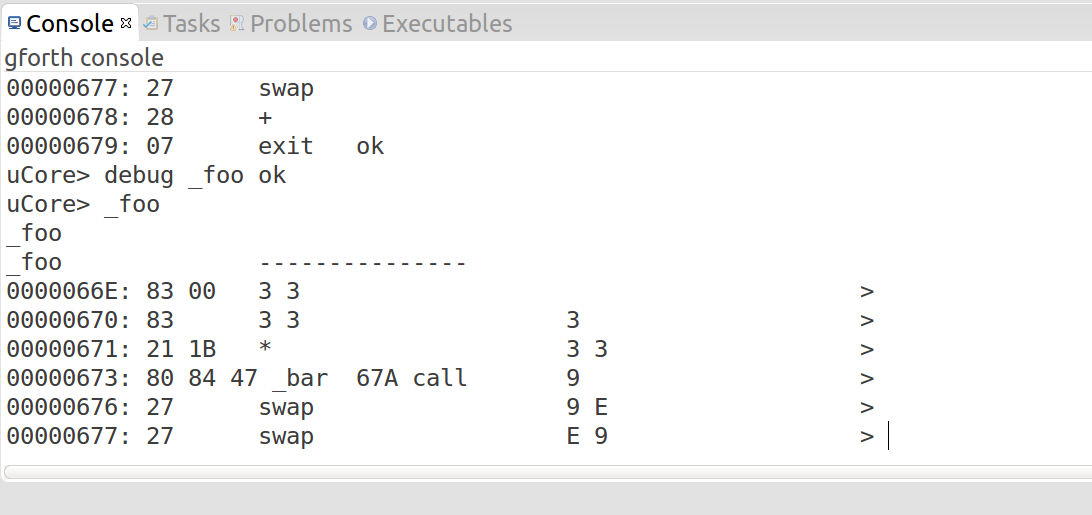
\includegraphics[scale=0.35]{debugger/consoledebugger.png}
		\caption{Konsolen basierter Debugger. Der Debugger kann über die Eclipse Console View gesteuert werden.}
		\captionsetup{margin=0cm,font={footnotesize}}
		\label{fig:extensionpoint}
\end{figure}

\section{Forth Debugger}

Eine weiter Möglichkeit ist, das Debug User Interface von Eclipse zu verwenden um den Debugger zu steuern. Dies ist für den Endanwender angenehmer, da  alle Informationen des Debuggers in einem User Interface ersichtlich sind.

\subsection{CDT oder JDT Debuggint Mechanismen}

Das Eclipse JDT stellt  mehrere Möglichkeiten zur Verfügung, wie ein Debugger integriert werden kann. Es können die vom Eclipse JDT verwendeten Mechanismen (vorallem das Plugin org.eclipse.debug.core), oder die vom CDT erweiterten Mechanismen (vorallem das Plugin org.eclipse.cdt.debug.core), welche verwendet werden um einen C oder C++ Debugger zu integrieren. Das vom CDT zur Verfügung gestellte Plugin wird vorallem dazu verwendet, um ein neuer C oder C++ Debugger zu integrieren, da es sich aber um einen Forth Debugger handelt, werden diese Erweiterungen nicht gebraucht. Ich habe mich deshalb dazu entschieden, das JDT Debugging zu verwenden.

\subsection{Debugger Aktionen}

Für den Debugger wurden einige Aktionen, welche schon im Eclipse verwendet werden, implementiert und einige neue Forth spezifische Aktionen hinzugefügt.

\subsubsection{Step}
Mit der Step Aktion kann ein normaler single step ausgeführt werden. Es wird dafür ein \verb! CR! Command an den Forth Prozess gesendet.
\begin{figure}[H]
	\centering
		
\includegraphics[scale=1]{debugger/step.png}
		\caption{Step Aktion.}
		\captionsetup{margin=0cm,font={footnotesize}}
		\label{fig:extensionpoint}
\end{figure}

\subsubsection{Step Into}

\begin{figure}[H]
	\centering
		
\includegraphics[scale=1]{debugger/stepinto.png}
		\caption{Konsolen basierter Debugger. Der Debugger kann über die Eclipse Console View gesteuert werden.}
		\captionsetup{margin=0cm,font={footnotesize}}
		\label{fig:extensionpoint}
\end{figure}

\subsubsection{Jump}

\subsubsection{Over}

\subsubsection{Terminate}

\begin{figure}[H]
	\centering
		
\includegraphics[scale=1]{debugger/terminate.png}
		\caption{Konsolen basierter Debugger. Der Debugger kann über die Eclipse Console View gesteuert werden.}
		\captionsetup{margin=0cm,font={footnotesize}}
		\label{fig:extensionpoint}
\end{figure}

\subsubsection{Kill}

\subsection{Stack View}

In der Stack View wird er aktuelle Dstack angezeigt. Die Stack View wird automatisch nach jedem steppen des Debuggers aktualisiert.

\begin{figure}[H]
	\centering
		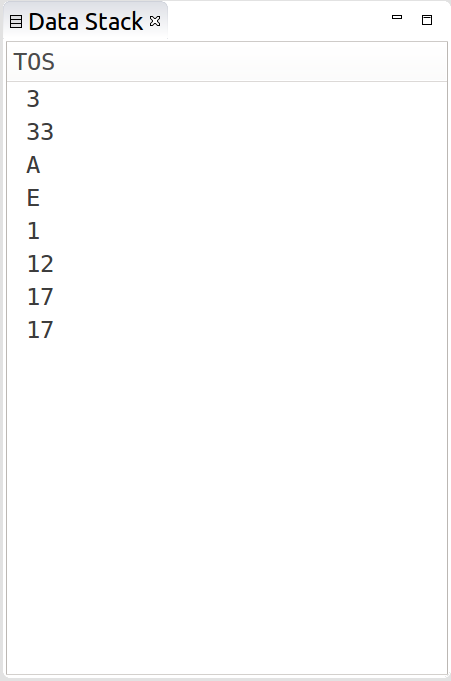
\includegraphics[scale=0.35]{debugger/stack.png}
		\caption{Stack View mit aktuellem Dstack Inhalt. Der Top Of Stack (TOS) ist zuoberst in der Liste.}
		\captionsetup{margin=0cm,font={footnotesize}}
		\label{fig:extensionpoint}
\end{figure}


\subsection{Memory View}

In der Memory View kann ein Memory Dump, welcher mit dem \verb! dump! Befehl von uForth abgefragt werden kann, angezeigt werden. Der Memory Dump wird automatisch nach jedem steppen des Debuggers aktualisiert.

\begin{figure}[H]
	\centering
		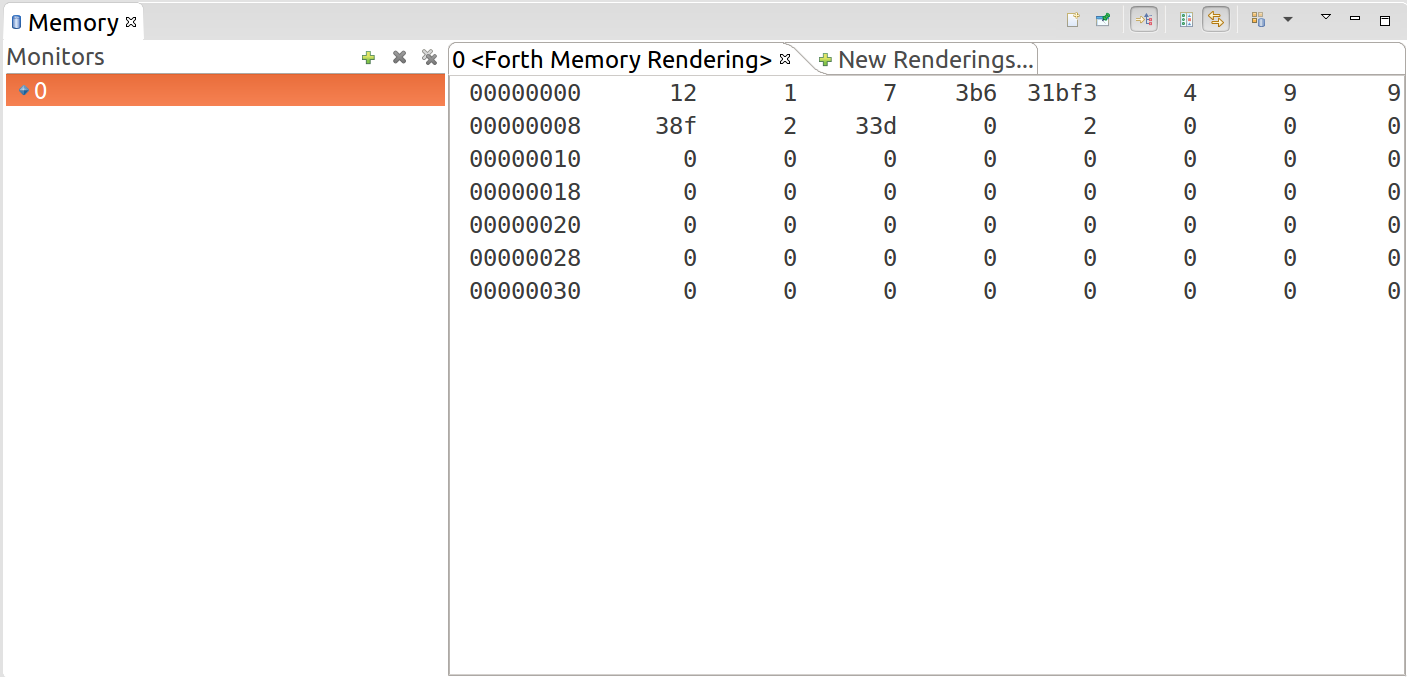
\includegraphics[scale=0.35]{debugger/dump.png}
		\caption{Eine Memory Dump, welcher}
		\captionsetup{margin=0cm,font={footnotesize}}
		\label{fig:extensionpoint}
\end{figure}


\section{C-Debugger}

Eine mögliche Erweiterung, wäre den Debugger so zu integrieren, das er direkt auf dem C-Source Code arbeitet (nicht wie bis jetzt, auf dem generierten Forth Code). Dies konnte nicht umgesetzt werden, da Debug Informationen des Compilers fehlen. Der C-Source Code kann nicht auf den entsprechenden generierten Forth Source Code abgebildet werden.
\chapter{Entwicklungsumgebungs Perference Page}
\label{chap:settings}
Für die Entwicklungsumgebung wurde eine Eclipse Preference Page erstellt. In diesem Kapitel wird erklärt, welche Einstellungen in dieser Preference Page vorgenommen werden können und welche Auswirkungen diese haben. Die Einstellungen sind im Eclipse Preference Dialog unter MCore zu finden.
\section{Umbilical Port}

Der Umbilical-Port kann über einen Dialog, der alle möglichen Ports anzeigt, ausgewählt werden.

\begin{figure}[H]
	\centering
		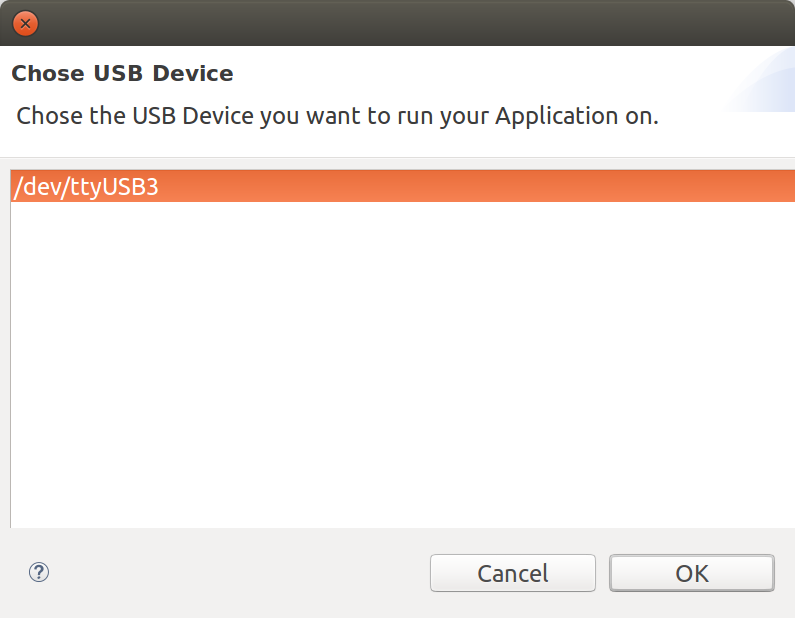
\includegraphics[scale=0.3]{idesettings/umbilical.png}
		\caption{Dialog, über welchen der Umbilical-Port gesetzt werden kann.}
		\captionsetup{margin=0cm,font={footnotesize}}
		\label{fig:umbilicalport}
\end{figure}

Der Port wird automatisch gesetzt, wenn das Programm ausgeführt wird. 

\section{Loader}

Der Loader ist das File, das von Forth mit dem Befehl
%
\begin{verbatim}
gforth ./loader.fs
\end{verbatim}
%
gestartet wird. Im Loader befindet sich ein Platzhalter \$INPUT\_FILE, der bei der Ausführung des Programms durch den Namen des Files ersetzt wird.
\chapter{Optimierungen}
\label{chap:optimizer}
In diesem Kapitel wird beschrieben, was für Optimierungen für den Compiler implementiert wurden. Im Forth Cross-Compiler sind schon einige Peephole Optimierungen implementiert. In diesem Kapitel werden die neu implementierten Optimierungen mit dessen des Cross-Compilers verglichen und gezeigt wo noch bessere Optimierungsstrategien verwendet werden können.

\section{Peephole Optimierung}

Peephole Optimierungen ist eine Art von Optimierung, welche auf einer kleinen Sequenz von Instruktionen durchgeführt wird. Dieses Sequenz wird Peephole oder auch Window genannt. Die Peephole Optimierung verucht Sets von Instruktionen durch kürzere oder schnellere Instruktionen zu ersetzen.\cite{peepwiki} Peephole Optimierungen können die grösse des Codes um 15--40 Prozent verkleinern und sind heute in allen gängigen Compilern implementiert.\cite{peepdavidson} Zu den Peephole Optimierungen gehören unter anderen folgende Arten von Optimierungen:

\begin{itemize} 
	\item Constant Folding - Konstante Expressions auswerten
	\item Constant Propagation - Konstante Werte in Expressions substituieren
	\item Strength Reduction - Langsame Instruktionen mit äquivalenten schnellen Instruktionen ersetzen.
	\item Combine Operations - Mehrere Oprationen mit einer äquivalenten ersetzen
	\item Null Sequences - Unötige Operationen entfernen\cite{peepwiki}
\end{itemize}

\newpage

\subsection{Beispiele}

Folgend einige Peephole Optimierungs Beispiele anhand von Forth Code.

\subsubsection{Constant Propagation}
\label{constantprogationsection}

Folgende Instruktionen
%
\begin{verbatim}
1
2
swap
+
dup
\end{verbatim}
%
können durch:
%
\begin{verbatim}
2
2
\end{verbatim}
%
ersetzt werden. Die Instruktionen swap, + und dup können schon zur Kompilierzeit durchgeführt werden.
\subsubsection{Combine Operations}
Folgende zwei Instruktionen
%
\begin{verbatim}
rot
rot
\end{verbatim}
%
können durch
%
\begin{verbatim}
-rot
\end{verbatim}
%
ersetzt werden. Die zwei rot Instruktionen sind äquivalent zu einer -rot Instruktion. Oder die folgenden zwei Instruktionen
%
\begin{verbatim}
dup
drop
\end{verbatim}
%
können durch
%
\begin{verbatim}
nop
\end{verbatim}
%
ersetzt werden. Die zwei Instruktionen heben sich auf und können somit entfernt werden.

\newpage

\subsection{Optimierungen}

Für den Compiler wurden Prototypen mässig zwei Optimierungen in Java implementiert. Die erste Optimierung versucht benachbarte Instruktionen zu vereinfachen. Die zweite Optimierung ist eine einfache Constant Propagation. Die beiden Optimierungen werden in den nächsten Kapiteln genauer beschrieben. Der neue Optimizer wird in zwei Phasen durchgeführt:

\begin{figure}[H]
	\centering
		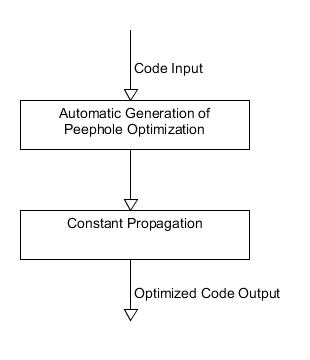
\includegraphics[scale=0.6]{optimizer/optimizer.png}
		\caption{Die zwei Phasen des Optimizers.}
		\captionsetup{margin=0cm,font={footnotesize}}
		\label{fig:optimizer}
\end{figure}

Im Cross-Compiler wurden unter anderem folgende Peephole Optimierungen schon implementiert.

\begin{enumerate}
  \item \verb!<lit> + ld, <lit> + st, <lit> + @!, and \verb!<lit> + \!! werden mit automatisch inkrementierenden Speicherzugriff Instruktionen ersetzt, wenn \verb!<lit>! sich zwischen \-4 und 3 befindet
  \item Folgende Stack Operationen: \\
				$swap, swap \rightarrow nop$\\
				$-rot, rot \rightarrow nop$\\
				$swap, + \rightarrow +$\\

\end{enumerate}

Für eine komplette Liste siehe "real time, object oriented with debugger" \cite{uforth}.

\newpage
\subsection{Automatische Generierung von Peephole Optimierungen}

Klassische Peephole Optimizer versuchen häufig einige Maschinenspezifische Patterns zu korrigieren. Der von Davidson und Fraser\cite{peepdavidson} beschriebene Algorithmus (PO) verwendet eine Machine Description, simuliert benachbarte Instruktionen und versucht diese mit äquivalenten, schnelleren Instruktionen zu ersetzen. Für den Forth Optimizer wurde ein Teil des PO objektorientiert implementiert.

\subsection{Constant Propagation}
Unter Constant Propagation versteht man, dass vorwärts substituieren von Konstanten im Code. Dies kann zur Folge haben, dass mehrere Instruktionen schon zur Kompilierzeit ausgewertet werden können, wie bei den Beispielen \ref{constantprogationsection} zu sehen ist.

\subsection{Resultate und Tests}
Die Resultate des Optimierers wurden mit verschiedenen Forth Funktionen getestet und die Resultate mit dem Peephole Optimizer des uForth Cross-Compilers verglichen. Der Source-Code zu den getesteten Funktionen befindet sich im Anhang.

\begin{table}[H]
\begin{center}
    \begin{tabular}{ | l | l | l | l | p{8cm} |}
    \hline
    \textbf{Funktion} & \textbf{Orig} & \textbf{Ref} & \textbf{Neu} & \textbf{Kommentar} \\ \hline
    \_Init & 126 & 112 & 119 & Die Referenzimplementierung produziert vor allem wegen der Speicherzugriffsoptimierung kürzeren Code. Constant Propagation, welche neu implementiert wurde, konnte keine durchgeführt werden. PO konnte Instruktionspaare finden, welche weg optimiert werden können.  \\ \hline
		\_Update & 8 & 8 & 4 & PO konnte zwei Instruktionspaare weg optimieren, welche von der Referenzimplementierung nicht optimiert werden. \\ \hline
		\_Hash & 65 & 60 & 60 & Die Referenzimplementierung produziert wieder wegen der Speicherzugriffsoptimierung weniger Code. PO konnte wieder Instruktionspaare finden, welche weg optimiert werden können. \\ \hline
		\_Propagation & 11 & 11 & 4 & Bei dieser Funktion konnte vor allem Constant Propagation durchgeführt werden. Die Referenzimplementierung führt keine Constant Propagation durch. \\ \hline
    \end{tabular}
		\caption{Resultate des neuen Optimizers verglichen mit dem Cross-Compiler Optimizer.}
		\label{tab:peepresults}
\end{center}
\end{table}
\newpage

Es hat sich herausgestellt, dass bei allen Beispielen die Constant Propagation nur wenig Code optimieren konnte. Dies ist vermutlich der Fall, weil konstante Ausdrücke schon vom Compiler optimiert werden und die implementierte Constant Propagation zu primitiv ist. Im nächsten Kapitel werden einige Erweiterungen vorgeschlagen, um diese effizienter zu gestalten.  

PO konnte Regeln finden, welche vom Forth-Cross Compiler noch nicht erkannt werden. Unter anderem folgende:\\ \\
%
$swap, swap \rightarrow nop$\\
$-rot, rot \rightarrow nop$\\
$rot, -rot \rightarrow nop$\\
$1, + \rightarrow 1+$\\
$swap, + \rightarrow +$\\
%

Diese Regeln könnten im Forth Cross-Compiler integriert werden. Im nächsten Kapitel werden Änderungen für den PO vorgeschlagen, damit dieser mehr mögliche Instruktionsketten erkennen könnte, welche vereinfacht werden können.

\subsection{Mögliche Erweiterungen}

Im Moment werden vom PO nur Insturktionen, welche einen Einfluss auf den Daten Stack haben simuliert. PO könnte erweitert werden, indem weitere Instruktionen auch simuliert werden. Eine weiter Möglichkeit wäre, der von Bansal und Aiken beschriebene Superoptimizer zu implementierten. Dieser Superoptimizer verwendet Bruteforce Optimierungen mittels tausenden von Regeln. Diese Regeln werden von Trainings Programmen inferiert und in einer Datenbank gespeichert.\cite{superoptimizer}

Die Constant Propagation könnte noch so erweitert werden, dass sie auch mit Branches umgehen kann. Somit könnten unnötige If-Statements, sowie Schleifen entfernt werden. Um dies zu implementieren müsste der Code zuerst in eine static single assignemt form (SSA) transformiert werden.\cite{ssa} Es wäre somit aber keine Peephole Optimierung mehr.

% schluss

\appendix


\bibliography{MicroCoreIDE}{}
\bibliographystyle{unsrt}
\newpage

\listoffigures
\listoftables

\newpage
\chapter{Ehrlichkeitserklärung}
Hiermit bestätigen die Autoren, diese Arbeit ohne fremde Hilfe und unter Einhaltung der gebotenen Regeln erstellt zu haben.
\\
\\
\\
\textbf{Benjamin Neukom}
\\
\\
\\
\rule{0.75\textwidth}{0.4pt} \\
Ort, Datum \hspace * {4cm} Unterschrift


\end{document}
